\documentclass{standalone}

\usepackage{tikz}

\usetikzlibrary{fit, calc, decorations, decorations.pathreplacing}

\begin{document}
  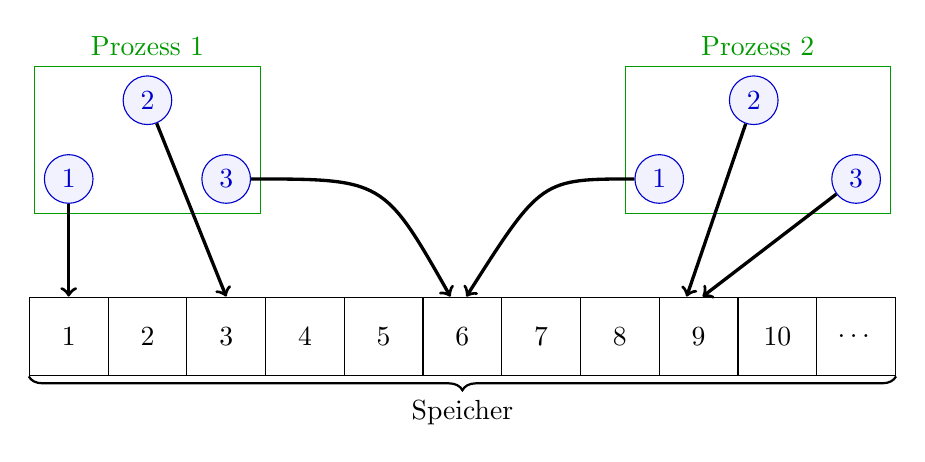
\begin{tikzpicture}[
    x=1mm, 
    y=1mm,
    selektor/.style={
      fill=blue!5!white, 
      text=blue!80!black,
      draw=blue!80!black,
      circle
    },
    task/.style={draw=green!60!black, text=green!60!black, rectangle},
    mempage/.style={draw, rectangle, minimum width=1cm, inner sep=0, minimum height=1cm}]
   \path
     node(pd11) at (  0, 0)  [selektor] {1}
     node(pd12) at ( 10,10)  [selektor] {2}
     node(pd13) at ( 20, 0)  [selektor] {3}
     node(pd21) at ( 75, 0)  [selektor] {1}
     node(pd22) at ( 87,10)  [selektor] {2}
     node(pd23) at (100, 0)  [selektor] {3};

   \node[task, label={[green!60!black]Prozess 1}, fit=(pd11) (pd12) (pd13)] {};
   \node[task, label={[green!60!black]Prozess 2}, fit=(pd21) (pd22) (pd23)] {};

   \foreach \x[count=\i] in {0,10,...,90}
     \node[mempage, at={(\x, -20)}](mem\i) {\i}; 
   \node[mempage, at={(100,-20)}](memlast){\dots};

   \begin{scope}[very thick]
     \draw[->] (pd11) -- (mem1.north);
     \draw[->] (pd12) -- (mem3.north);
     \draw[->] (pd13) .. controls (40,0) .. ($(mem6.north west)!.35!(mem6.north east)$);
     \draw[->] (pd21) .. controls (60,0) .. ($(mem6.north west)!.55!(mem6.north east)$);
     \draw[->] (pd22) -- ($(mem9.north west)!.35!(mem9.north east)$);
     \draw[->] (pd23) -- ($(mem9.north west)!.55!(mem9.north east)$);
   \end{scope}

   \draw[decorate, decoration={brace, amplitude=5}, thick]
     (memlast.south east) -- (mem1.south west);
   \node[at=($(memlast.south east)!.5!(mem1.south west)$), anchor=north, yshift=-5]
     {Speicher}; 
  \end{tikzpicture}
\end{document}
